\documentclass[a4paper, 12pt]{article}

\usepackage{tikz}
\usetikzlibrary{automata, positioning, arrows}
\usepackage{float}

\usepackage{xcolor}
\usepackage[left=2cm, right=2cm, top=2cm, bottom=2cm]{geometry}

\usepackage{ mathrsfs }

\usepackage{amsmath}

\tikzset{
	->,
	node distance=3cm, 
	>=stealth',
	every state/.style={thick},
	baseline}

\begin{document}
\pagenumbering{roman}
\title{
		\textbf{Group Members}\\ 
		Tevin Achong - 816000026\\
		Jimmel Greer - 816000045\\
		\textbf{Course Code:} COMP3602\\
		\textbf{Course Title:} Theory of Computing\\
		\textbf{Assignment:} 2
		\date{November 21, 2019}
}
\maketitle

\newpage
\begin{enumerate}
\item ~

\begin{itemize}
\item
$L = \{1^n0^{\frac{n}{2}}$ $\vert$ $n \geq 2$, n is even$\}$\\
$G = (\{S\}, \{0, 1\}, P, S)$\\
where $P$ is:\\
S $\rightarrow$ 11S0 $\vert$ 110

\item
$\{+w+w^R+$ $\vert$ $w \in \{0,1\}^+\}$\\
$G = (\{S, W\}, \{+, 0, 1\}, P, S)$\\
where $P$ is:\\
S $\rightarrow$ $+W+$\\
W $\rightarrow$ 1W1 $\vert$ 0W0 $\vert$ 1+1 $\vert$ 0+0\\

\item
$\{w+v$ $\vert$ $w, v \in \{0,1\}^*,$ $w^R$ is the prefix of $v\}$\\
G = (\{S, W, V\}, \{+, 0, 1, $\epsilon$\}, P, S)\\
where $P$ is:\\
S $\rightarrow$ WV $\vert$ $\epsilon$ $+$ $\epsilon$\\
W $\rightarrow$ 1W1 $\vert$ 0W0 $\vert$ 1+1 $\vert$ 0+0\\
V $\rightarrow$ 0V $\vert$ 1V $\vert$ $\epsilon$\\

\vspace{3cm}
\end{itemize}

\item ~
\begin{itemize}
\item ~
$\{1^n0^{\frac{n}{2}}$ $\vert$ $n \geq 2$, n is even$\}$
\begin{figure}[H]
	\centering
	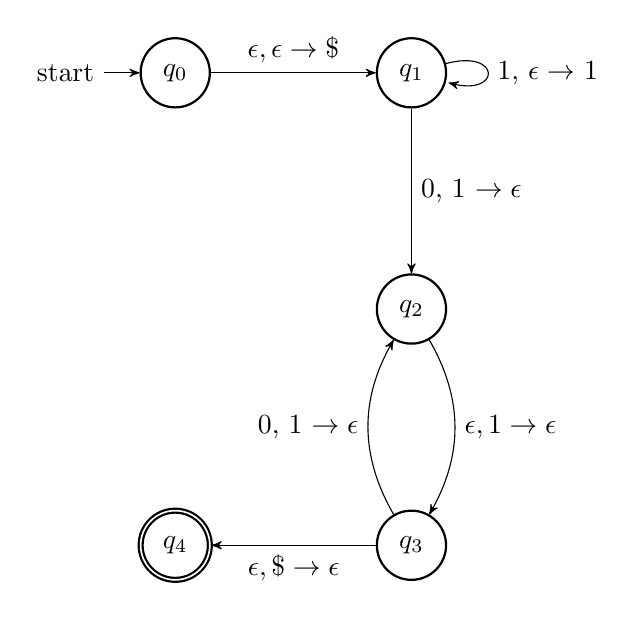
\begin{tikzpicture}
		
		\node[state, initial] (q0) {$q_0$};
		\node[state, right of=q0] (q1) {$q_1$};
		\node[state, below of=q1] (q2) {$q_2$};
		\node[state, below of=q2] (q3) {$q_3$};
		\node[state, accepting, left of=q3] (q4) {$q_4$};
		
		\draw 
		(q0) edge[above] node{$\epsilon , \epsilon \rightarrow \$$} (q1)
		(q1) edge[loop right, right] node{1, $\epsilon \rightarrow$ 1} (q1)
		(q1) edge[right] node{0, 1 $\rightarrow \epsilon$} (q2)
		(q2) edge[bend left, right] node{$\epsilon , 1 \rightarrow \epsilon$} (q3)
		(q3) edge[bend left, left] node{0, 1 $\rightarrow \epsilon$} (q2)
		(q3) edge[below] node{$\epsilon , \$ \rightarrow \epsilon$} (q4)
		;
	\end{tikzpicture}
\end{figure}

\item ~
$\{+w+w^R+$ $\vert$ $w \in \{0,1\}^+\}$
\begin{figure}[H]
	\centering
	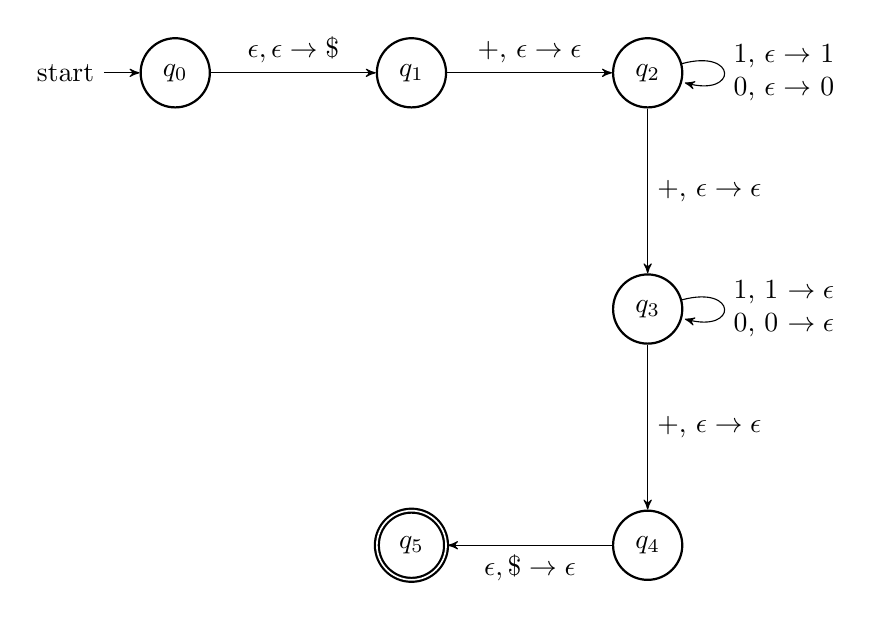
\begin{tikzpicture}
		
		\node[state, initial] (q0) {$q_0$};
		\node[state, right of=q0] (q1) {$q_1$};
		
		\node[state, right of=q1] (q2) {$q_2$};		
		\path[->] (q2) edge[loop right, right] node[align=center] {1, $\epsilon \rightarrow$ 1\\0, $\epsilon \rightarrow$ 0} (q2);		
		
		\node[state, below of=q2] (q3) {$q_3$};
		\path[->] (q3) edge[loop right, right] node[align=center] {1, 1 $\rightarrow \epsilon$\\0, 0 $\rightarrow \epsilon$} (q3);
		
		\node[state, below of=q3] (q4) {$q_4$};
		\node[state, accepting, left of=q4] (q5) {$q_5$};
		
		\draw 
		(q0) edge[above] node{$\epsilon , \epsilon \rightarrow \$$} (q1)
		(q1) edge[above] node{+, $\epsilon \rightarrow \epsilon$} (q2)
		(q2) edge[right] node{+, $\epsilon \rightarrow \epsilon$} (q3)
		(q3) edge[right] node{+, $\epsilon \rightarrow \epsilon$} (q4)
		(q4) edge[below] node{$\epsilon , \$ \rightarrow \epsilon$} (q5)
		;
	\end{tikzpicture}
\end{figure}

\newpage
\item ~
$\{w+v$ $\vert$ $w, v \in \{0,1\}^*,$ $w^R$ is the prefix of $v\}$
\begin{figure}[H]
	\centering
	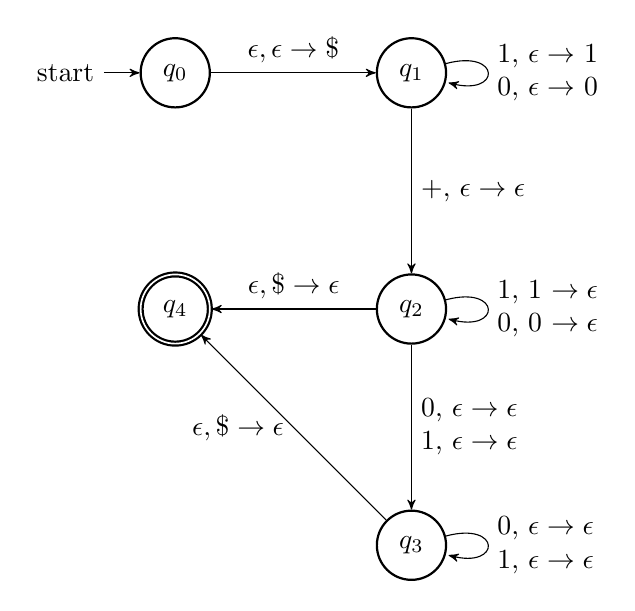
\begin{tikzpicture}
		
		\node[state, initial] (q0) {$q_0$};
		
		\node[state, right of=q0] (q1) {$q_1$};
		\path[->] (q1) edge[loop right, right] node[align=center] {1, $\epsilon \rightarrow$ 1\\0, $\epsilon \rightarrow$ 0} (q1);
		
		\node[state, below of=q1] (q2) {$q_2$};		
		\path[->] (q2) edge[loop right, right] node[align=center] {1, 1 $\rightarrow \epsilon$\\0, 0 $\rightarrow \epsilon$} (q2);
		
		
		\node[state, below of=q2] (q3) {$q_3$};
		\path[->] (q3) edge[loop right, right] node[align=center] {0, $\epsilon \rightarrow \epsilon$\\1, $\epsilon \rightarrow \epsilon$} (q3);
		\path[->] (q2) edge[right] node[align=center] {0, $\epsilon \rightarrow \epsilon$\\1, $\epsilon \rightarrow \epsilon$} (q3);
		
		\node[state, accepting, left of=q2] (q4) {$q_4$};

		
		\draw 
		(q0) edge[above] node{$\epsilon , \epsilon \rightarrow \$$} (q1)
		(q1) edge[right] node{+, $\epsilon \rightarrow \epsilon$} (q2)
		(q2) edge[above] node{$\epsilon , \$ \rightarrow \epsilon$} (q4)
		(q3) edge[left] node{$\epsilon , \$ \rightarrow \epsilon$} (q4)
		
		;
	\end{tikzpicture}
\end{figure}
\end{itemize}

\newpage
\item
If $L_1$ and $L_2$ are any context-free languages, $L_1 \cup L_2$ is also context free.\\
\textbf{Proof by Construction:}\\
If $L_1$ and $L_2$ are context free, then, by definition, there exist grammars $G_1 = (V_1, \Sigma_1, S_1, P_1)$ and $G_2 = (V_2, \Sigma_2, S_2, P_2)$ with $L(G_1) = L_1$ and $L(G_1) = L_1$. We can assume that $V_1$ and $V_2$ are disjoint. Now consider the grammar $G = (V, \Sigma, S, P)$, where $S$ is a new nonterminal symbol and\\
\indent
$V = V_1 \cup V_2 \cup \{S\}$,\\
$\Sigma = \Sigma_1 \cup \Sigma_2$, and\\
$P = P_1 \cup P_2 \cup \{(S \rightarrow S_1), (S \rightarrow S_2)\}$\\

Clearly $L(G) = L_1 \cup L_2$, so $L_1 \cup L_2$ is a regular language.

\item
If $L$ is any context-free language, $L^*$ is also context free.\\
\textbf{Proof by Construction:}\\
If $L$ is context free then, by definition, there exists a grammar $G = (V, \Sigma, S, P)$ with $L(G) = L$. Now consider the grammar $G' = (V', \Sigma', S', P')$, where $S'$ is a new nonterminal symbol and\\
$V' = V \cup \{S'\}$, and\\
$P' = P \cup \{(S' \rightarrow SS'), (S' \rightarrow \epsilon)\}$\\

Now $L(G') = L^*$, so $L^*$ is a context-free language.


\newpage
\item 
\begin{itemize}
\item[(a)]
\textbf{Non-terminals:}\\
$R, S, T, X$

\item[(b)]
\textbf{Terminals:}\\
$a, b, \epsilon$

\newpage
\item[(c)] ~
\textbf{Parse Tree for $abb$}
\begin{figure}[H]
	\centering
	\begin{tikzpicture}
		
		\node[state] (q0) {$R$};
		\node[state, below of=q0] (q1) {$S$};
		\node[state, below of=q1] (q2) {$T$};
		\node[state, left of=q2] (q3) {$a$};
		\node[state, right of=q2] (q4) {$b$};
		\node[state, below of=q2] (q5) {$X$};
		\node[state, below of=q5] (q6) {$b$};		
				
		\draw 
		(q0) edge[] node{} (q1)
		(q1) edge[] node{} (q2)
		(q1) edge[] node{} (q3)
		(q1) edge[] node{} (q4)
		(q2) edge[] node{} (q5)
		(q5) edge[] node{} (q6)
		;
			
		
	\end{tikzpicture}
\end{figure}


\item[(d)] ~
\textbf{Derivation of $bba$:}\\
$R \Rightarrow S \Rightarrow bTa \Rightarrow bXa \Rightarrow bba$

\end{itemize}


\end{enumerate}
\end{document}